\section{Implementation}
\label{sec:impl}
We have chosen to implement a monitoring system for Node.js based on \emph{code instrumentation}.
The core idea is to modify the original source code of the program to be monitored in a way that allows observation of relevant events.
Once an event is observed, the monitor can verify it against the specification, eventually acting in case of erroneous behavior.

The tool we have employed is \emph{Jalangi2} \cite{jalangi}.
% gia' linkato nelle prime pagine
%\footnote{\url{https://github.com/Samsung/jalangi2}} \cite{jalangi}
It allows addition of arbitrary code before and after basically every JavaScript operation: access to fields, declarations, functions and methods invocation, among others. Jalangi2 also gives access to information about the operation itself, as the arguments of a function call or the target object of a field access.
The tool allows for state-of-the-art performance in the context of code instrumentation for dynamic analysis.
To the best of our knowledge, the most similar tool is Linvail \cite{linvail}, though its performance are reported to be worst by an order of magnitude (w.r.t.\ the overhead).

Thanks to these features it is possible to determine when asynchronous calls and their callbacks are executed, as well as matching them.
However, implementing a prototype for Node.js runtime verification is not trivial, and requires to address some issues, as explained below:
\begin{itemize}
\item Anonymous functions are extremely common in JavaScript, thus function names are not a reliable way to identify them.
\item Matching asynchronous functions with their callback needs some bookkeeping: the same asynchronous function can be used multiple times with different arguments and callbacks, and vice versa.
In order to deal with this problem, our prototype dynamically wraps callbacks \emph{at runtime} and generate a unique identifier for each one of them.
\item The prototype only tracks the program, but does not directly interact with the Node.js runtime.
Since the execution goes back and forth between the event loop and the program, tracking the flow is not easy.
\item Many different patterns arise in Node.js programming, and they need complex code instrumentation.
For instance, the file system module functions expect a file descriptor as an argument, while HTTP requests are handled through methods invoked on objects encoding the requests.
\end{itemize}
Our prototype implementation enriches the capabilities of Jalangi by supporting these additional features that for Node.js monitoring.
We are currently working on a proxy-based alternative approach based on reflection rather than instrumentation.
Proxies \cite{proxy} are currently natively supported by JavaScript.

The current implementation of trace expression semantics is coded in SWI-Prolog, since logic programming is a natural fit for inference rules and transition systems, and cyclic terms are supported by the \texttt{coinduction} library \cite{CoLP06}.

Our monitoring system has two main parts.
On one hand, an instrumented Node.js program is executed, and the additional code observes relevant events.
On the other hand, a Prolog server encoding the trace expression specification is running and validating events.
These two parts communicate through a HTTP interface, and events are exchanged in the JSON format.
The architecture is represented in \Cref{fig:arch}.
Further details on the approach and the implementation with Jalangi2 can be found in the related paper \cite{TowardsIoT17}.

Though JSON is a natural fit for JavaScript objects serialization, some important aspects need to be handled.
Objects containing circular references, for instance, are quite common in Node.js modules, but they cannot be encoded in JSON, and the JavaScript standard library serialization (\lstinline|JSON.stringify|) throws an error on such objects.
Furthermore, JavaScript supports getters, which are special functions invoked when a property is accessed.
During experiments, we found that some modules set getter functions before their code can actually be correctly executed, and this again breaks standard serialization since getters are invoked in the process.
For these reasons, we had to modify the JSON serialization process for it to work in real Node.js scenarios, detecting and handling circular references and getters as special cases.

This work is a preliminary step towards runtime verification of Internet of Things applications,
both because Node.js is emerging as a standard framework for IoT development, and the implementation through an HTTP
server offers a natural support to verification of distributed systems, where (instrumented) devices can send events to a monitoring server.

\begin{figure}
\centering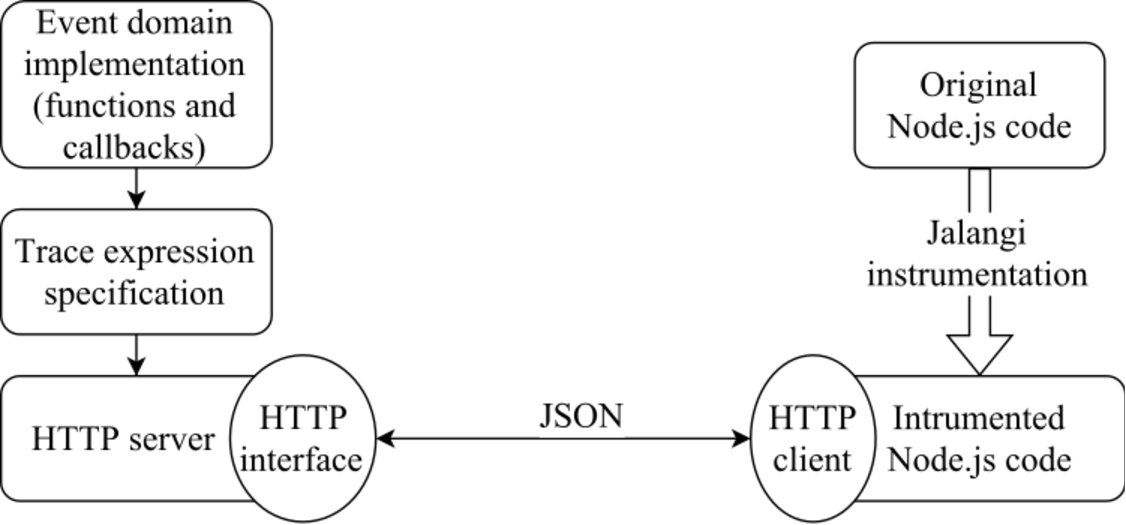
\includegraphics[width=.7\textwidth]{fig/diagram}
\caption{Monitoring architecture for Node.js exploiting SWI-Prolog server with an HTTP interface.}
\label{fig:arch}
\end{figure}

